% Template for ICIP-2018 paper; to be used with:
%          spconf.sty  - ICASSP/ICIP LaTeX style file, and
%          IEEEbib.bst - IEEE bibliography style file.
% --------------------------------------------------------------------------
\documentclass{article}
\usepackage{spconf,amsmath,graphicx}
\usepackage{amsthm}
\usepackage{hyperref}

\newtheorem{definition}{Definition}
\newtheorem{theorem}{Theorem}
\newtheorem{proposition}{Proposition}
\newtheorem{corollary}{Corollary}
\newtheorem{lemma}{Lemma}
\newtheorem{exercise}{Exercise}
\newtheorem{example}{Example}

\DeclareMathOperator*{\argmin}{arg\,min}
\DeclareMathOperator*{\argmax}{arg\,max}
\DeclareMathOperator*{\Val}{\text{Val}}
\DeclareMathOperator*{\Ch}{\text{Ch}}
\DeclareMathOperator*{\Pa}{\text{Pa}}
\DeclareMathOperator*{\Sc}{\text{Sc}}
\newcommand{\ov}{\overline}
\newcommand{\tsup}{\textsuperscript}

% Example definitions.
% --------------------
\def\x{{\mathbf x}}
\def\L{{\cal L}}

% Title.
% ------
\title{VISUALIZING GENERATIVE SUM-PRODUCT NETWORKS ON IMAGE RECONSTRUCTION}
% Single address.
% ---------------
\name{Renato L. Geh}
\address{University of São Paulo\\Institute of Mathematics and Statistics\\
  Rua do Matão, 1010 - São Paulo, SP, Brazil, 05508-090}
%
% For example:
% ------------
%\address{School\\
%	Department\\
%	Address}
%
% Two addresses (uncomment and modify for two-address case).
% ----------------------------------------------------------
%\twoauthors
%  {A. Author-one, B. Author-two\sthanks{Thanks to XYZ agency for funding.}}
%	{School A-B\\
%	Department A-B\\
%	Address A-B}
%  {C. Author-three, D. Author-four\sthanks{The fourth author performed the work
%	while at ...}}
%	{School C-D\\
%	Department C-D\\
%	Address C-D}
%
\begin{document}
%\ninept
%
\maketitle
%
\begin{abstract}
  Sum-Product Networks (SPNs) are fairly recent deep tractable probabilistic graphical models that
  are able to answer exact queries in linear time. Although there have been many advancements in
  practical problems, there is an absence in literature of visualizations on how SPNs represent
  learned data. In this paper we show how two structure learning algorithms can heavily impact on
  how SPNs treat data, particularly in the domain of image reconstruction. We show two coloring
  techniques to visualize sum and product nodes through their scopes. We then apply both techniques
  to generative SPNs learned from two distinct learning methods.
\end{abstract}
%
\begin{keywords}
Sum-product networks, probabilistic graphical models, visualization, image reconstruction
\end{keywords}
%
\section{Introduction}
\label{sec:intro}

Image reconstruction is the task of accurately predicting, guessing and completing missing elements
from an image. Density estimators that model a joint probability distribution can achieve this by
learning the features of similar images and finding the valuation that most adequately fits the
incomplete image. However, classical density estimators, such as Probabilistic Graphical Models
(PGMs), suffer from exact inference intractability in the general case. This leads to approximate
prediction and representation, as learning in PGMs often requires the use of inference as a
subroutine.

Sum-Product Networks (SPNs)~\cite{poon11} are fairly recent tractable PGMs capable of representing
distributions as a deep network of sums and products. Most importantly, SPNs are capable of exact
inference in time linear to its graph's edges. There have been many advances on SPNs in the image
domain, such as image classification and reconstruction~\cite{gens13,dennis12,gens12}, image
segmentation~\cite{yuan16} and activity recognition~\cite{amer12,amer16,wang18}. However, there
have been little effort~\cite{vergari16} so far to explore SPNs' semantics and representation
power.

In this paper, we provide visualizations on SPNs learned from two structure learning algorithms. We
present two techniques to perform this task. These techniques rely on a couple of properties SPNs
must follow in order to correctly represent a probability distribution, and are highly dependent on
the graph's structure. We first give a short background review of SPNs, relevant properties and
scope definition. We follow this with an explanation on how we achieved the visualizations shown in
this article. Finally, we show results and provide a conclusion of our findings.

%In this paper, we provide visualizations on SPNs learned from the LearnSPN learning
%algorithm~\cite{gens13}, which we will call G-SPNs, and from the Dennis and Ventura clustering
%algorithm~\cite{dennis12}, mentioned here as D-SPNs.

\section{Background}
\label{sec:back}

An SPN can be seen as a DAG with restrictions with respect to its node types and weighted edges.
Let $n$ be a graph node. The set of nodes $\Pa(n)$ and $\Ch(n)$ are the parents and children of
$n$. A weighted edge $i\to j$ is denoted by $w_{i,j}$.

\begin{definition}
  A sum-product network (SPN) is a directed acyclic graph. A node $n$ of an SPN can either be a:
  \begin{enumerate}\setlength\itemsep{0em}
    \item sum, where its value is given by $v_n=\sum_{j\in\Ch(n)}w_{n,j}v_j$;
    \item product, where its value is given by $v_n=\prod_{j\in\Ch(n)}v_j$;
    \item probability distribution, whose value is its probability of evidence.
  \end{enumerate}
\end{definition}

In this paper, we assume that all SPN leaves (i.e. node type 3) are tractable univariate
distributions, that is, computing its mode or partition function takes constant time. The scope of
a node $\Sc(n)$ is the union set of the scope of its children.

\begin{definition}[Completeness]
  An SPN is complete iff every child of a sum node has the same scope as its siblings.
\end{definition}

\begin{definition}[Decomposability]
  An SPN is decomposable iff every child of a product node has disjoint scope with its siblings.
\end{definition}

A complete and decomposable SPN correctly computes the probability of evidence of the modeled
distribution. An SPN that correctly represents a probability distribution is said to be valid. In
fact, a complete and consistent (i.e. no two children of an SPN node have contradicting variable
values) SPN is sufficient (though not necessary) for validity~\cite{poon11}. However,
learning decomposable SPNs is easier, and it has been shown that decomposability is as expressive
as consistency~\cite{peharz15}.

Let $\mathbf{X}=\{X_1=x_1,X_2,=x_2,\ldots,X_n=x_n\}$ be a valuation and $S$ an SPN. The value of
$S$ is the value of its root, and is denoted by $S(\mathbf{X})$. Inference in SPNs is done through
a bottom-up evaluation. The value of a leaf node $n$ is the probability of $\mathbf{X}$. If
$\Sc(n)\not\subset\mathbf{X}$, then $n$'s value is the distribution's mode.

Finding the $\argmax_{\mathbf{x}} S(\mathbf{X}=\mathbf{x})$, also called the Most Probable
Explanation (MPE), of an SPN has been shown to be NP-hard~\cite{peharz15,mei18,conaty17}. Image
reconstruction can be seen as an application of MPE, where each variable is a pixel, and values are
pixel colors. Finding the MPE, and thus the reconstruction of an image given some initial evidence
consists of finding the pixel values that are most likely to fit the model. Given that finding the
exact valuation that maximizes the model is hard, we instead use an approximate method proposed
in~\cite{poon11} called the Max-Product algorithm.

\begin{figure}[t]
  \centering\centerline{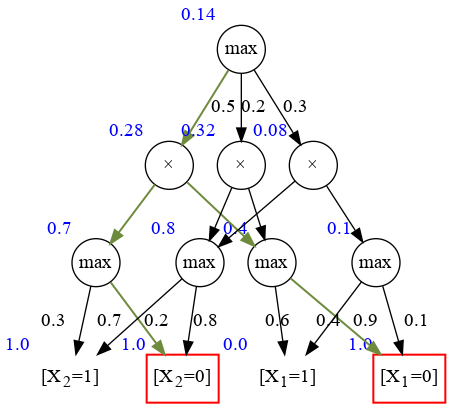
\includegraphics[width=0.45\textwidth]{imgs/sample_mpn_prob.png}}
  \caption{Finding the MPE of an SPN given $\mathbf{X}=\{X_1=0\}$.\label{fig:mpn}}
\end{figure}

The Max-Product algorithm consists of replacing the original SPN with a Max-Product Network (MPN).
An MPN of an SPN is simply the SPN with its sum nodes replaced with max nodes. The value of a max
node is the maximum weighted child. Finding an MPE approximation on an MPN is done through a
bottom-up evaluation similar to an SPN. Once all nodes have been computed, a top-down traversal is
done, finding the max paths in the graph by choosing only the max edge in a max node and traversing
all edges in product nodes, as shown in~\autoref{fig:mpn}.

\section{Visualizing SPNs}
\label{sec:visual}

Visualization in SPNs can be done through an analysis of the SPN's scope and structure. The
definition of completeness lends itself naturally to an interpretation of sum nodes as layers of
mixture models. A possible intuition for this interpretation is that sum nodes model latent
variables in charge of explaining similar interactions between variables. Decomposability, on the
other hand, models independence between sets of variables.



\section{Results}
\label{sec:results}

\section{Conclusion}
\label{sec:conc}

% Below is an example of how to insert images. Delete the ``\vspace'' line,
% uncomment the preceding line ``\centerline...'' and replace ``imageX.ps''
% with a suitable PostScript file name.
% -------------------------------------------------------------------------
%\begin{figure}[htb]

%\begin{minipage}[b]{1.0\linewidth}
  %\centering
  %\centerline{\includegraphics[width=8.5cm]{image1}}
%%  \vspace{2.0cm}
  %\centerline{(a) Result 1}\medskip
%\end{minipage}
%%
%\begin{minipage}[b]{.48\linewidth}
  %\centering
  %\centerline{\includegraphics[width=4.0cm]{image3}}
%%  \vspace{1.5cm}
  %\centerline{(b) Results 3}\medskip
%\end{minipage}
%\hfill
%\begin{minipage}[b]{0.48\linewidth}
  %\centering
  %\centerline{\includegraphics[width=4.0cm]{image4}}
%%  \vspace{1.5cm}
  %\centerline{(c) Result 4}\medskip
%\end{minipage}
%%
%\caption{Example of placing a figure with experimental results.}
%\label{fig:res}
%%
%\end{figure}


% To start a new column (but not a new page) and help balance the last-page
% column length use \vfill\pagebreak.
% -------------------------------------------------------------------------
%\vfill
%\pagebreak

% References should be produced using the bibtex program from suitable
% BiBTeX files (here: strings, refs, manuals). The IEEEbib.bst bibliography
% style file from IEEE produces unsorted bibliography list.
% -------------------------------------------------------------------------
\bibliographystyle{IEEEbib}
\bibliography{strings,refs}

\end{document}
